\documentclass[11pt,a4paper,titlepage]{article}
\usepackage[a4paper]{geometry}
\usepackage[utf8]{inputenc}
\usepackage[english]{babel}
\usepackage{lipsum}
\usepackage{eurosym}
\usepackage{rotating}

\usepackage{amsmath, amssymb, amsfonts, amsthm, mathtools}
% mathtools for: Aboxed (put box on last equation in align envirenment)
\usepackage{microtype} %improves the spacing between words and letters

\usepackage{lipsum}
\usepackage{threeparttable}
\usepackage{tabularx}
\usepackage{multirow}
\usepackage{booktabs}
\newcommand{\tabitem}{~~\llap{\textbullet}~~}
\usepackage{graphicx}
\graphicspath{ {./figures/} {./eps/}}
\usepackage{epsfig}
\usepackage{epstopdf}
\usepackage{verbatim}
\usepackage{textcomp}
\usepackage{tikz}
\usetikzlibrary{shapes,arrows}

%%%%%%%%%%%%%%%%%%%%%%%%%%%%%%%%%%%%%%%%%%%%%%%%%%
%% COLOR DEFINITIONS
%%%%%%%%%%%%%%%%%%%%%%%%%%%%%%%%%%%%%%%%%%%%%%%%%%
 % Enabling mixing colors and color's call by 'svgnames'
%%%%%%%%%%%%%%%%%%%%%%%%%%%%%%%%%%%%%%%%%%%%%%%%%%
\definecolor{MyColor1}{HTML}{CC0000} %mix personal color
\newcommand{\textb}{\color{Black} \usefont{OT1}{lmss}{m}{n}}
\newcommand{\blue}{\color{MyColor1} \usefont{OT1}{lmss}{m}{n}}
\newcommand{\blueb}{\color{MyColor1} \usefont{OT1}{lmss}{b}{n}}
\newcommand{\red}{\color{LightCoral} \usefont{OT1}{lmss}{m}{n}}
\newcommand{\green}{\color{Turquoise} \usefont{OT1}{lmss}{m}{n}}
%%%%%%%%%%%%%%%%%%%%%%%%%%%%%%%%%%%%%%%%%%%%%%%%%%


%%%%%%%%%%%%%%%%%%%%%%%%%%%%%%%%%%%%%%%%%%%%%%%%%%
%% FONTS AND COLORS
%%%%%%%%%%%%%%%%%%%%%%%%%%%%%%%%%%%%%%%%%%%%%%%%%%
%    SECTIONS
%%%%%%%%%%%%%%%%%%%%%%%%%%%%%%%%%%%%%%%%%%%%%%%%%%
\usepackage{titlesec}
\usepackage{sectsty}
%%%%%%%%%%%%%%%%%%%%%%%%
%set section/subsections HEADINGS font and color
\sectionfont{\color{MyColor1}}  % sets colour of sections
\subsectionfont{\color{MyColor1}}  % sets colour of sections

%set section enumerator to arabic number (see footnotes markings alternatives)
\renewcommand\thesection{\arabic{section}.} %define sections numbering
\renewcommand\thesubsection{\thesection\arabic{subsection}} %subsec.num.

%define new section style
\newcommand{\mysection}{
\titleformat{\section} [runin] {\usefont{OT1}{lmss}{b}{n}\color{MyColor1}}
{\thesection} {3pt} {} }

%%%%%%%%%%%%%%%%%%%%%%%%%%%%%%%%%%%%%%%%%%%%%%%%%%
%		CAPTIONS
%%%%%%%%%%%%%%%%%%%%%%%%%%%%%%%%%%%%%%%%%%%%%%%%%%
\usepackage{caption}
\usepackage{subcaption}
%%%%%%%%%%%%%%%%%%%%%%%%
\captionsetup[figure]{labelfont={color=MyColor1}}

%%%%%%%%%%%%%%%%%%%%%%%%%%%%%%%%%%%%%%%%%%%%%%%%%%
%		!!!EQUATION (ARRAY) --> USING ALIGN INSTEAD
%%%%%%%%%%%%%%%%%%%%%%%%%%%%%%%%%%%%%%%%%%%%%%%%%%
%using amsmath package to redefine eq. numeration (1.1, 1.2, ...)
%%%%%%%%%%%%%%%%%%%%%%%%
\renewcommand{\theequation}{\thesection\arabic{equation}}

%set box background to grey in align environment
\usepackage{etoolbox}% http://ctan.org/pkg/etoolbox
\makeatletter
\patchcmd{\@Aboxed}{\boxed{#1#2}}{\colorbox{black!15}{$#1#2$}}{}{}%
\patchcmd{\@boxed}{\boxed{#1#2}}{\colorbox{black!15}{$#1#2$}}{}{}%
\makeatother
%%%%%%%%%%%%%%%%%%%%%%%%%%%%%%%%%%%%%%%%%%%%%%%%%%

\newcommand{\DP}[1]{\textcolor{blue}{\textbf{(DP says: #1)}}}
\newcommand{\cri}[1]{\textcolor{green}{\textbf{(Cri says: #1)}}}

\makeatletter
\let\reftagform@=\tagform@
\def\tagform@#1{\maketag@@@{(\ignorespaces\textcolor{red}{#1}\unskip\@@italiccorr)}}
\renewcommand{\eqref}[1]{\textup{\reftagform@{\ref{#1}}}}
\makeatother
\usepackage[hidelinks]{hyperref}

%% LISTS CONFIGURATION %%
\usepackage{enumitem}
\setlist[enumerate,1]{start=0}
\renewcommand{\labelenumii}{\theenumii}
\renewcommand{\theenumii}{\theenumi.\arabic{enumii}.}

\usepackage[acronym]{glossaries}
\newacronym[plural=GEO,longplural={Geostationary Earth Orbits}]{geo}{GEO}{Geostationary Earth Orbit}
\newacronym[plural=LEO,longplural={Low Earth Orbits}]{leo}{LEO}{Low Earth Orbit}
\newacronym[plural=MEO,longplural={Medium Earth Orbits}]{meo}{MEO}{Medium Earth Orbit}
\newacronym[plural=HEO,longplural={High Elliptical Orbits}]{heo}{HEO}{High Elliptical Orbit}
\newacronym{eci}{ECI}{Earth Centered Inertial}
\newacronym{lla}{LLA}{geodetic latitude, longitude, altitude coordinates}
\newacronym[plural=GS,longplural={Ground Stations}]{gs}{GS}{Ground Station}
\newacronym{raan}{RAAN}{Right Ascending of Ascension Node}
\newacronym{eirp}{EIRP}{Effective Isotropic Radiated Power}
\newacronym{eol}{EOL}{End Of Life}

%%%%%%%%%%%%%%%%%%%%%%%%%%%%%%%%%%%%%%%%%%%%%%%%%%
%% PREPARE TITLE
%%%%%%%%%%%%%%%%%%%%%%%%%%%%%%%%%%%%%%%%%%%%%%%%%%
\title{\blue Eytu project}
\author{Davide Peron\\ Cristina Gava}
\date{\today}
%%%%%%%%%%%%%%%%%%%%%%%%%%%%%%%%%%%%%%%%%%%%%%%%%%

\begin{document}
\maketitle

\tableofcontents
\clearpage

\section{Power supply}
On the Wii U motherboard there is a discrete number of components involved in the power supply section, there are both passive components, discrete semiconductors and Integrated circuits all working together to power the PCB. In \autoref{tab:power} we summarized the main components listed under type and name: we can see the huge amount of passive components needed to support the integrated circuits and the discrete amount of transistors and diodes; on the other hand the number of integrated circuit is restrained.

\subsection{Integrated circuits description}
The three main integrated components that are worth to be described are:
\begin{itemize}
\item \textit{The power management IC}, model TPS65070RSL from Texas Instruments;
\item \textit{The Regulator DC/DC Converter, Step-Up}, model AIC1634GG from Analog Integration corp.;
\item \textit{The switchig Regulator DC/DC Controller, Step-Down}, model LV5066V from ON Semiconductors.
\end{itemize}

\begin{figure}
\centering
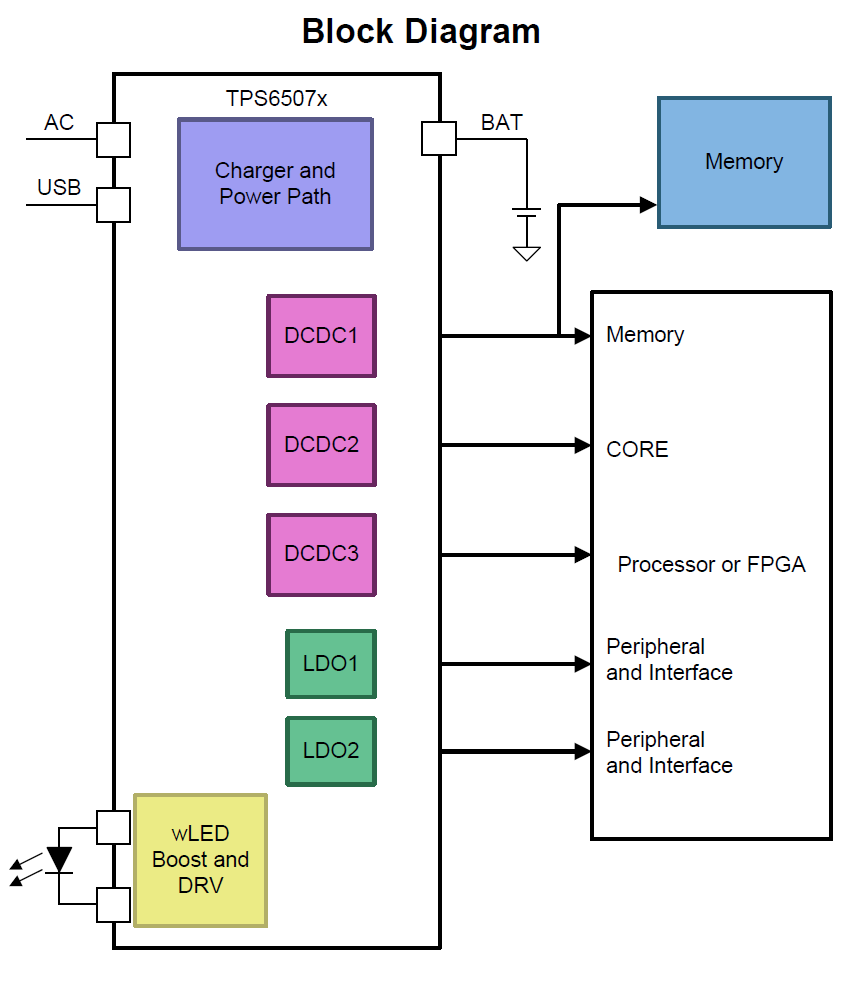
\includegraphics[width = .7\textwidth]{power_managIC.png}
\caption{Schematic for TPS65070RSL}
\label{fig:TPS65070RSL}
\end{figure}

\begin{table}
\centering
\begin{tabular}{llr}
\toprule
\textbf{Component type} & \textbf{Name} & \textbf{Qty}\\
\midrule
Integrated circuit & & \\
 & Regulator & 7\\
 & Analog IC & 5\\
 & Voltage Detector & 1\\
 & Power Manag. IC & 1\\
\hline
Discrete Semiconductor & &\\
 & Diode & 30\\
 & Transistor & 35\\
\hline
Passive comp. & &\\
 & Capacitor & 176\\
 & Fuse & 1\\
 & Ferrite Bead & 6\\
 & Inductor & 16\\
 & Resistor & 148\\ 
\bottomrule
\end{tabular}
\caption{Power supply component list}
\label{tab:power}
\end{table}


\bibliographystyle{IEEEtran}
\bibliography{IEEEabrv,bibliography}

\end{document}
